\documentclass[12pt, oneside]{report}

\usepackage[a4paper,right=20mm,left=30mm, top=30mm, bottom=20mm]{geometry}
\usepackage[utf8]{inputenc}
\usepackage[spanish]{babel}

% Imatges
\usepackage{graphicx, wrapfig}
\graphicspath{ {img/} }

% Bibliografia
\usepackage[style=numeric,backend=biber]{biblatex}
\addbibresource{bibliografia.bib}

% Profunditat del índex
\setcounter{tocdepth}{3}

% Lletra tipus Arial
\usepackage[OT1]{fontenc}
%\renewcommand*\familydefault{\sfdefault}

% Control de l'interlineat
\usepackage{setspace}
\setlength{\parskip}{\baselineskip}


\title{Elaboració d'un TDR amb \LaTeX{}}

\author{
  Otero Mateo, Noé\\
  \texttt{noe.otero@gmail.com}
}
\author{
  De Tal, Fulano\\
  \texttt{fulanodetal@gmail.com}
}

\begin{document}

% Portada
\maketitle

% Índex
\tableofcontents

\onehalfspace

% Agraiments (opcional)
\chapter*{Agradecimientos}
% Aquest capítol es no numerat. S'ha d'afegir manualment a l'índex.
\addcontentsline{toc}{chapter}{Agradecimientos}
Aqui van els agraïments del TDR. Aprofita per tot el que vulguis agrair!

% Introducció
\chapter*{Introducción}
% Aquest capítol es no numerat. S'ha d'afegir manualment a l'índex.
\addcontentsline{toc}{chapter}{Introducción}
En esta investigación, exploramos la historia y situación actual de la divulgación científica, desde sus comienzos en el siglo XVII hasta hoy en día. Examinamos críticamente las prácticas y tendencias actuales en divulgación científica, evaluando su impacto y capacidad para satisfacer las necesidades informativas del público. También nos proponemos investigar las razones subyacentes detrás de la falta de información científica básica en la sociedad contemporánea. Nos sumergiremos en las posibles causas que contribuyen a esta carencia, desde deficiencias en los sistemas educativos hasta barreras de acceso a la información.


%------------------------------------------------------------------
%
%                        COS DEL TREBALL
%
%------------------------------------------------------------------
\chapter{Historia de la divulgación científica}
\label{cap:primer}
Aqui tenin cites al famós article d'Einstein \autocite{Einstein05}, al que podria ser el millor llibre de l'historia \Autocite{GMMarquez67} i al article de Wikipedia sobre \LaTeX{} \autocite{Wikipedia_LaTeX}.

A continuació, anem a veure com incloure figures i il.lustracions. La figura \ref{fig:gos} mostra un goset ben aixerit.
\begin{figure}[h]
    \centering
    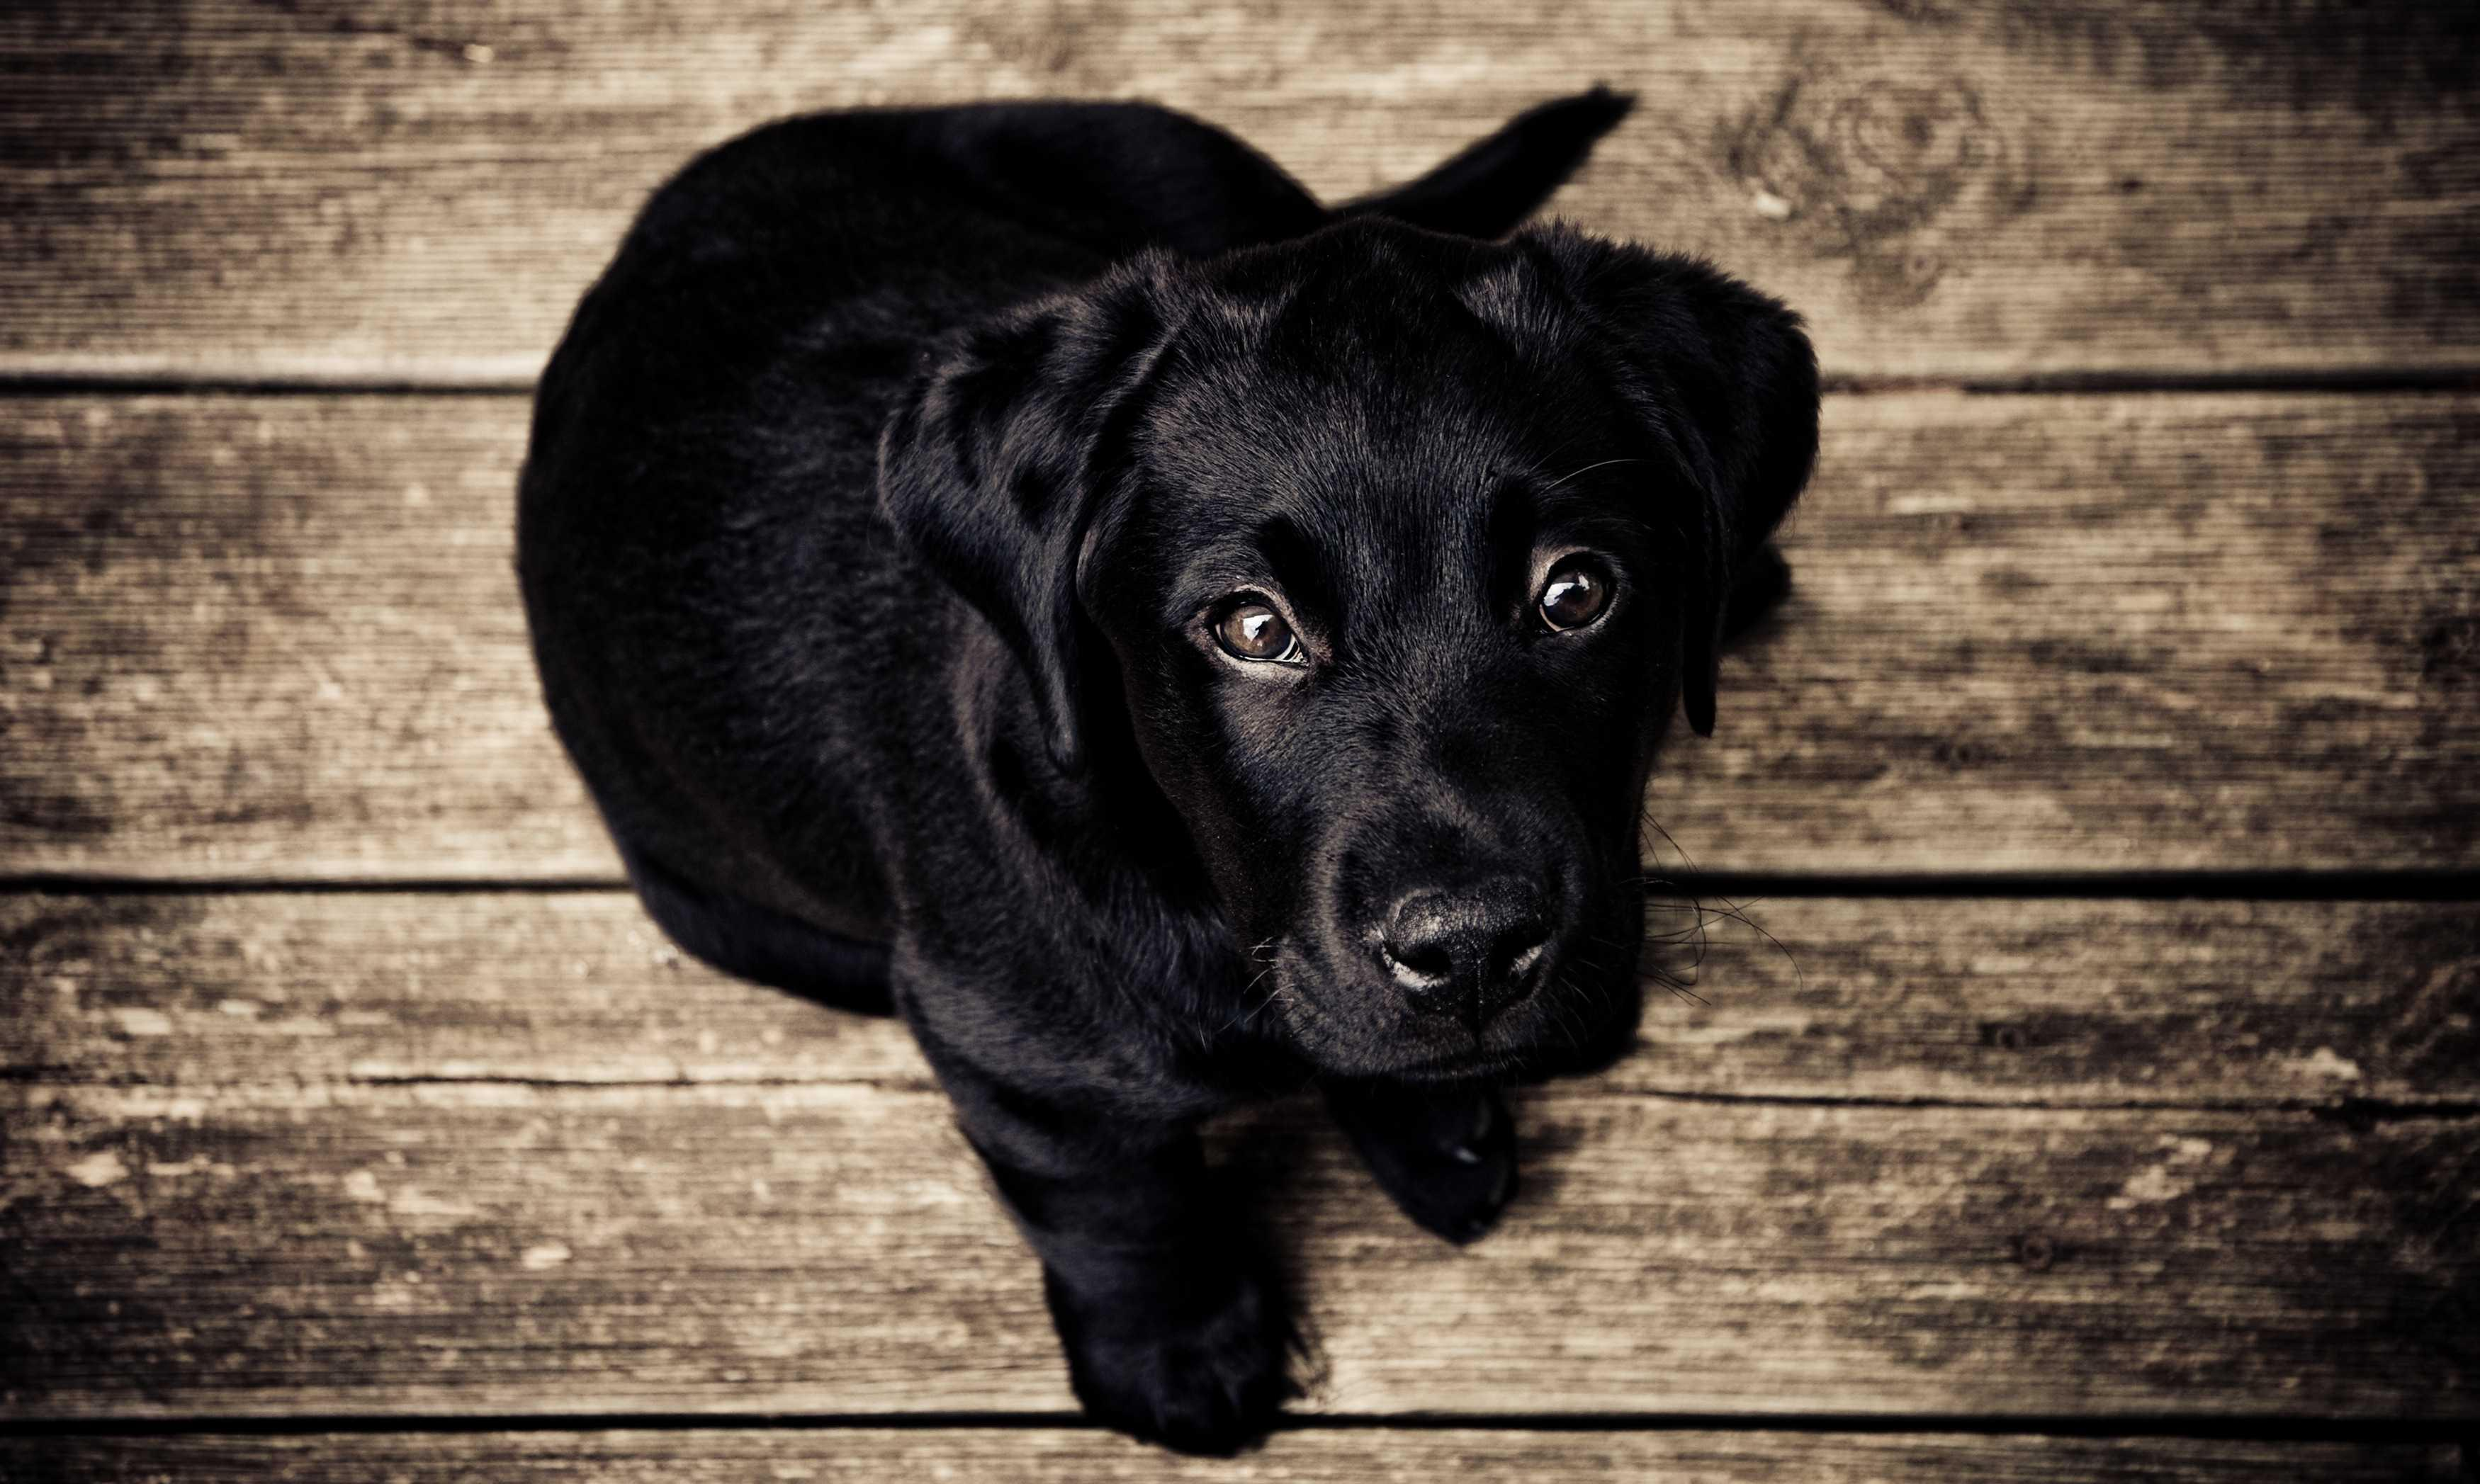
\includegraphics[width=0.55\textwidth]{random_img_04}
    \caption{Un goset qualsevol}
    \label{fig:gos}
\end{figure}

\begin{wrapfigure}{l}{0.25\textwidth}
    \centering
    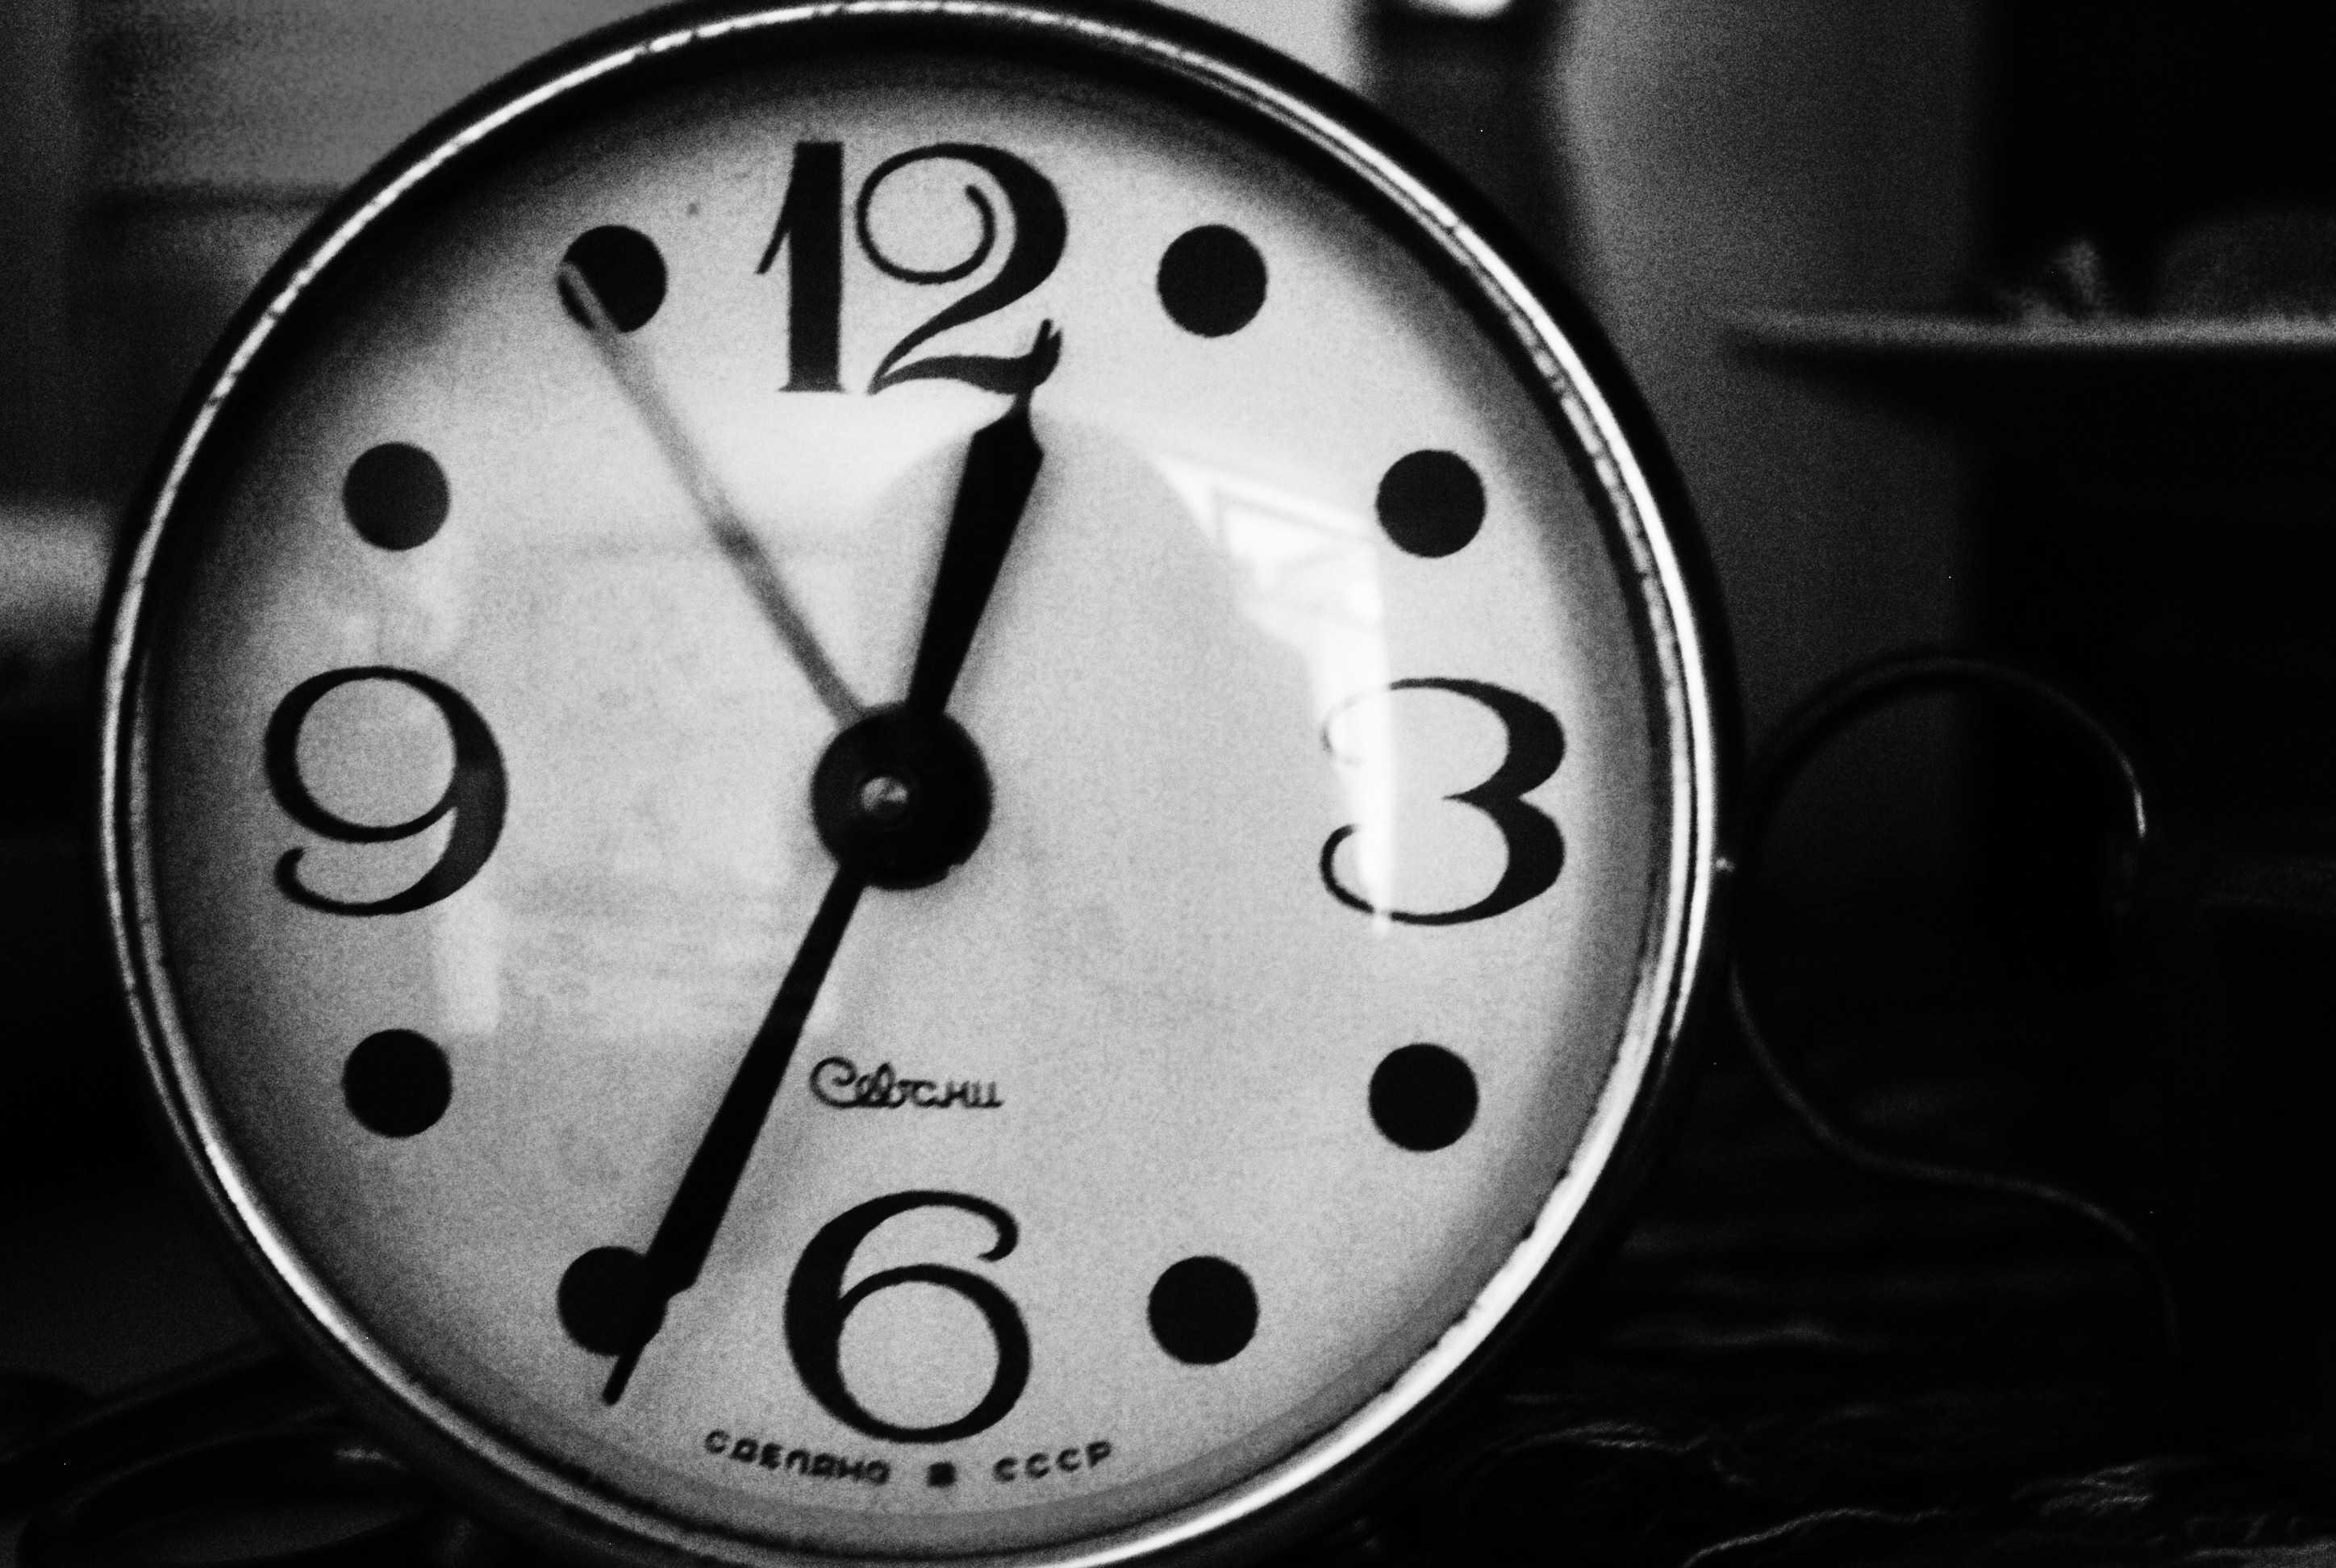
\includegraphics[width=0.25\textwidth]{random_img_03}
    \caption{El temps vola}
    \label{fig:rellotge}
\end{wrapfigure}

De vegades, per això, volem que l'imatge estigui insertada al text, que també es pot fer, com es pot veure a la figura \ref{fig:rellotge}. A continiuació, una mica de text sense sentir per omplir espai. Pulvinar elementum integer enim neque volutpat ac tincidunt vitae. Turpis massa sed elementum tempus egestas sed sed. Mauris sit amet massa vitae tortor. Vel turpis nunc eget lorem dolor sed. Nullam ac tortor vitae purus faucibus. Ornare suspendisse sed nisi lacus. Urna porttitor rhoncus dolor purus non. Sed faucibus turpis in eu. Dictum at tempor commodo ullamcorper a lacus vestibulum sed arcu. Commodo elit at imperdiet dui accumsan sit amet. Sit amet porttitor eget dolor morbi. Tellus in metus vulputate eu scelerisque felis imperdiet. Risus nullam eget felis eget nunc.

\begin{wrapfigure}{r}{0.5\textwidth}
    \centering
    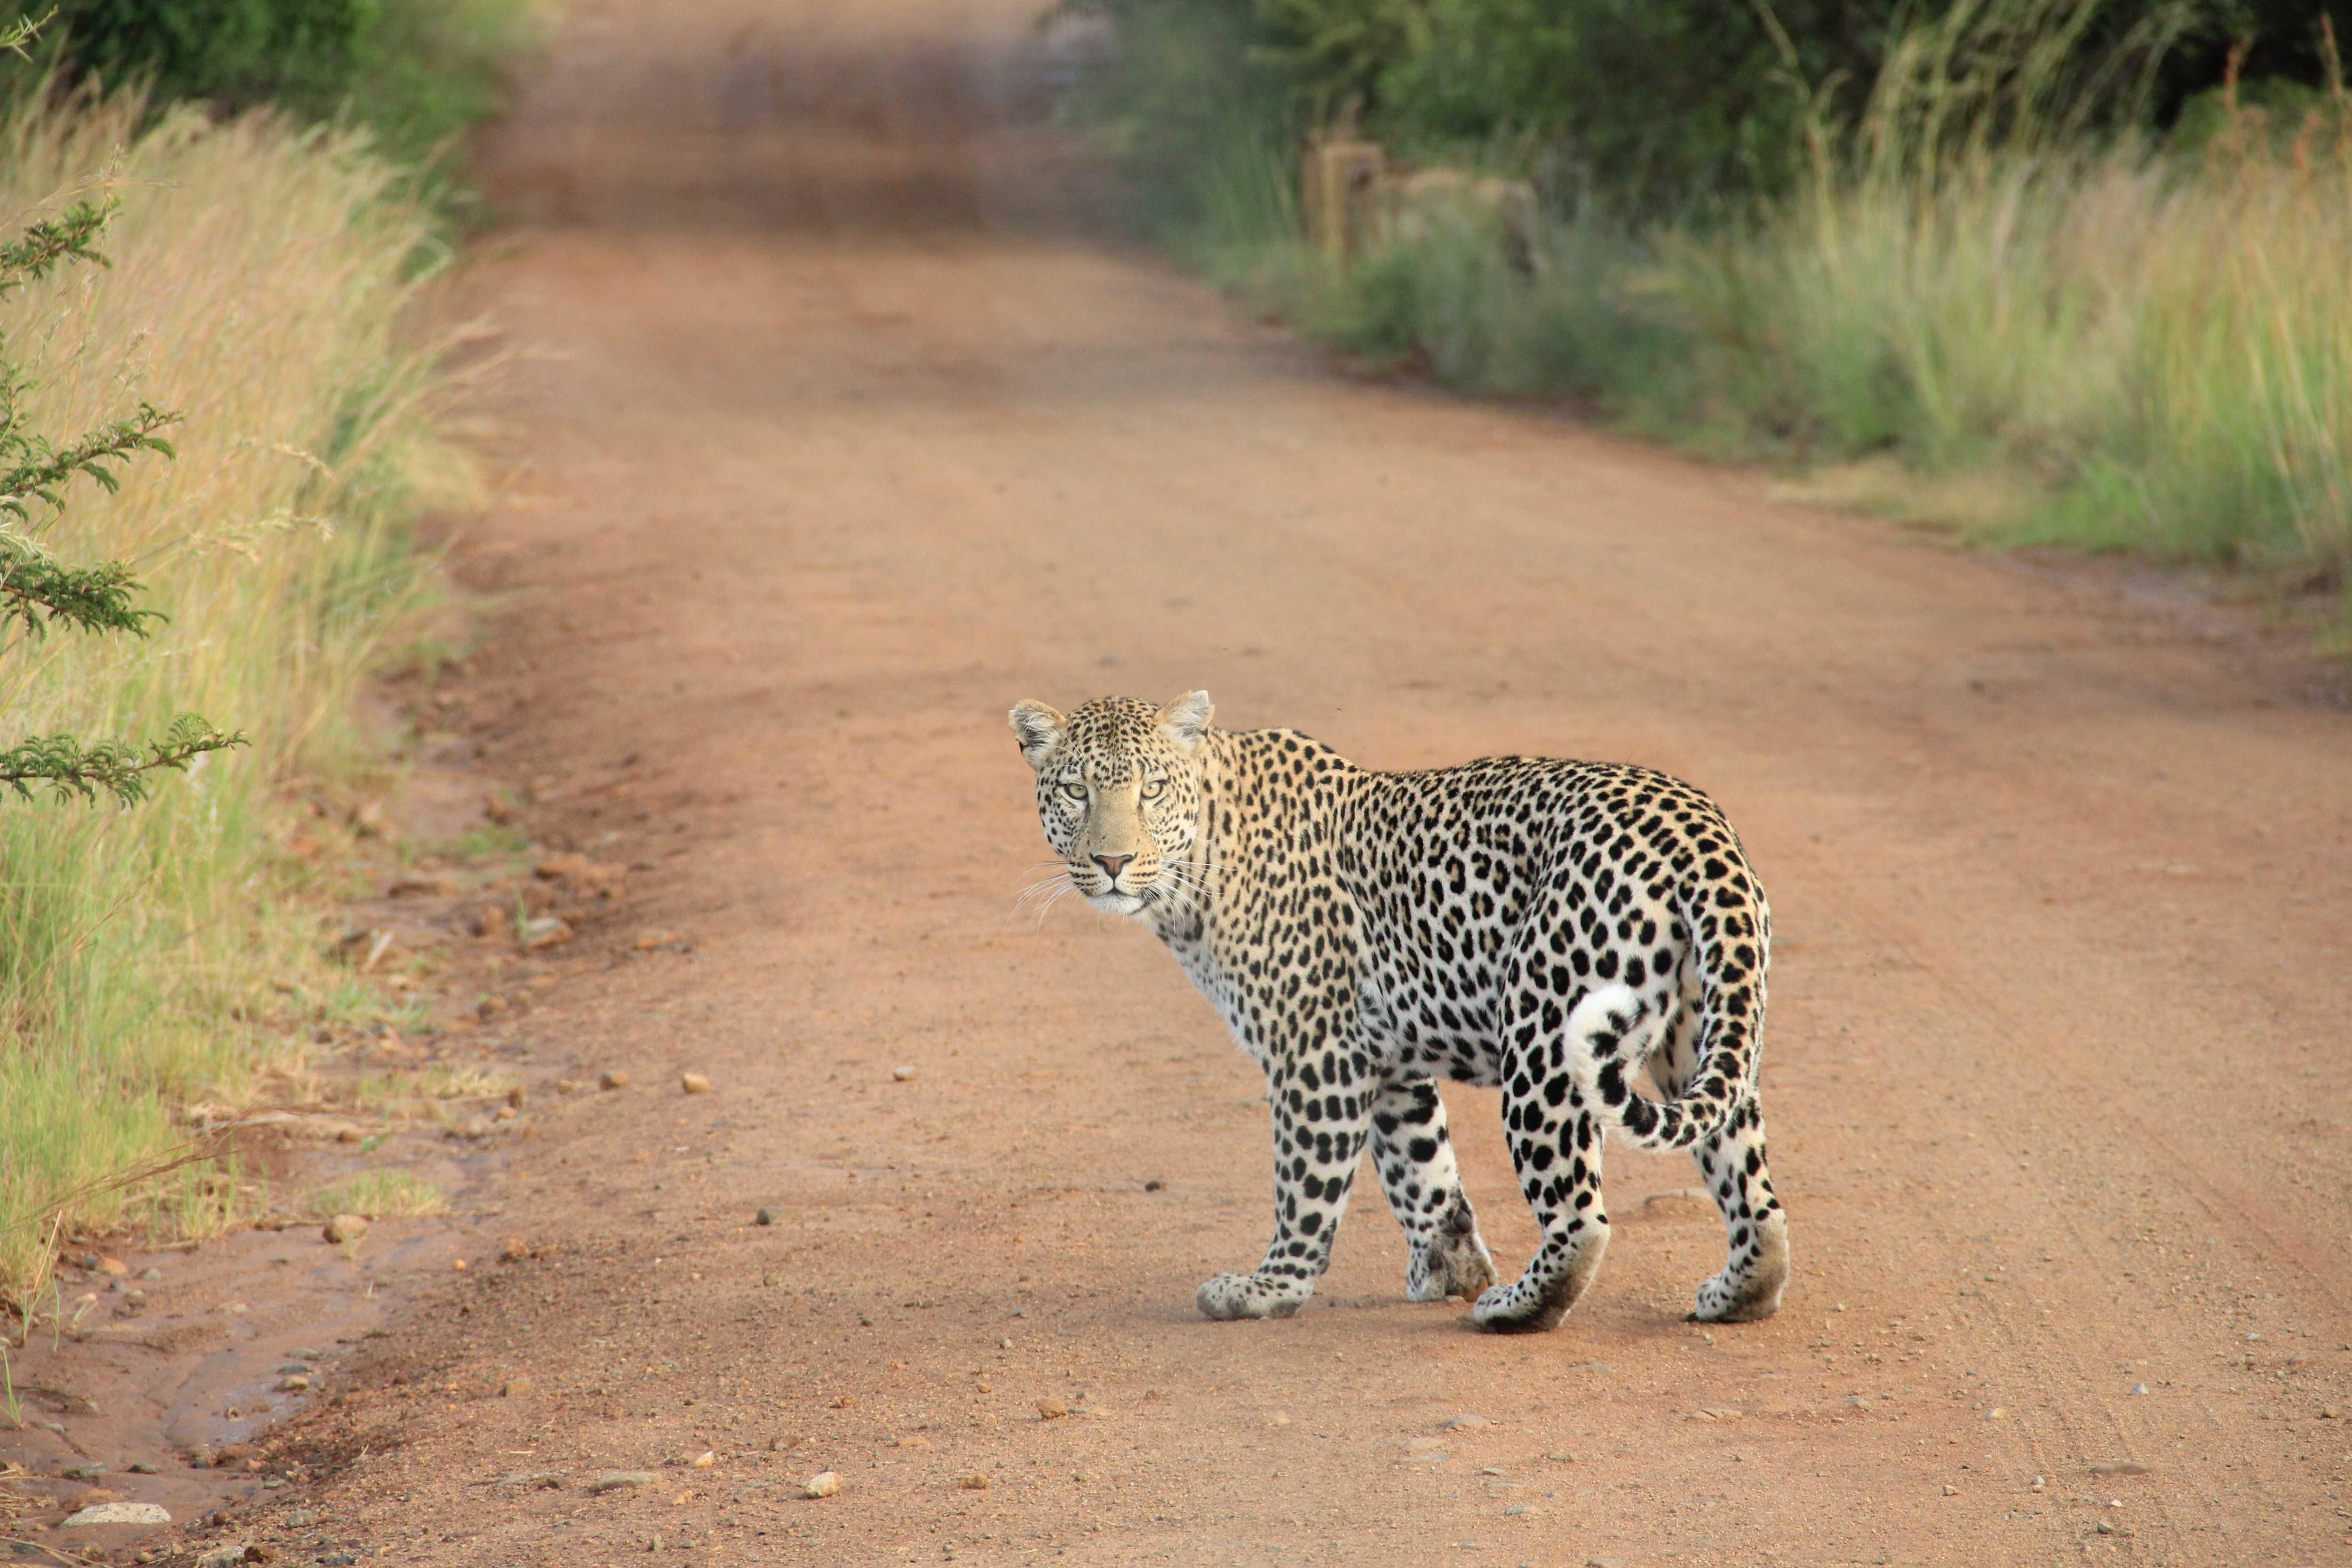
\includegraphics[width=0.95\linewidth]{random_img_05}
    \caption{El lleopard}
    \label{fig:lleopard}
\end{wrapfigure}
També es pot alinear a la dreta com es pot observar a la figura \ref{fig:lleopard}. Erat imperdiet sed euismod nisi porta. Ut porttitor leo a diam sollicitudin tempor id eu nisl. Ante in nibh mauris cursus. In nibh mauris cursus mattis molestie a iaculis at. Tempus imperdiet nulla malesuada pellentesque. Eget duis at tellus at urna condimentum mattis. Blandit turpis cursus in hac. Egestas integer eget aliquet nibh. Lobortis elementum nibh tellus molestie. Morbi tincidunt augue interdum velit euismod. Vestibulum sed arcu non odio euismod lacinia. Fermentum leo vel orci porta. Cursus sit amet dictum sit amet justo donec enim diam. Fermentum iaculis eu non diam phasellus vestibulum. Eleifend mi in nulla posuere sollicitudin aliquam. Volutpat commodo sed egestas egestas fringilla phasellus faucibus scelerisque. Justo donec enim diam vulputate ut pharetra sit.

Per ultim, potser volem inserir una taula com la de la taula \ref{taula:preus_menjar} seguent.
\begin{table}[h!]
\centering
\begin{tabular}{|c|c|l|}
    \hline
    Producte & Descripció & Preu \\
    \hline
    Patates & Per fregir & 3,25 \\
    Espàrrecs & Per truita & 1,12 \\
    Pà & Per torrar i fer sopa & 2,25 \\
    \hline
\end{tabular}
\caption{Els preus del menjar.}
\label{taula:preus_menjar}
\end{table}

\section{Siglo XVII: Orígenes de la divulgación científica}
Dignissim suspendisse in est ante in nibh mauris cursus mattis. Libero enim sed faucibus turpis in eu. Nunc mi ipsum faucibus vitae aliquet nec ullamcorper. Nam at lectus urna duis convallis convallis tellus id interdum. Lacus suspendisse faucibus interdum posuere lorem ipsum dolor sit. Urna cursus eget nunc scelerisque viverra mauris in aliquam sem. Magna fringilla urna porttitor rhoncus dolor. Etiam dignissim diam quis enim lobortis. Amet justo donec enim diam vulputate. Aenean pharetra magna ac placerat vestibulum lectus mauris ultrices. Nibh ipsum consequat nisl vel pretium lectus. Orci sagittis eu volutpat odio facilisis mauris. Hac habitasse platea dictumst vestibulum rhoncus est. Tellus orci ac auctor augue mauris.

\section{Siglo XVIII: La Ilustración y las sociedades científicas}
Lorem ipsum dolor sit amet, consectetur adipiscing elit, sed do eiusmod tempor incididunt ut labore et dolore magna aliqua. Nisl nisi scelerisque eu ultrices vitae. Ligula ullamcorper malesuada proin libero nunc consequat interdum varius sit. Libero justo laoreet sit amet cursus sit. Cursus eget nunc scelerisque viverra mauris in. Egestas pretium aenean pharetra magna ac. Urna molestie at elementum eu facilisis sed. Mi tempus imperdiet nulla malesuada pellentesque. Lectus proin nibh nisl condimentum id venenatis a condimentum. Adipiscing at in tellus integer feugiat. Cursus risus at ultrices mi tempus.

\section{Siglo XIX: El surgimiento de la divulgación moderna}
Donec ac odio tempor orci. In est ante in nibh mauris cursus mattis. Et egestas quis ipsum suspendisse ultrices gravida. In fermentum posuere urna nec tincidunt. Interdum posuere lorem ipsum dolor. Sit amet cursus sit amet dictum sit. Sit amet consectetur adipiscing elit pellentesque. Quis lectus nulla at volutpat. Sit amet volutpat consequat mauris nunc. Et netus et malesuada fames ac turpis egestas maecenas.

\section{Siglo XX: La edad de ero de la divulgación Científica}
Diam vel quam elementum pulvinar etiam non quam. Non diam phasellus vestibulum lorem sed risus. Integer eget aliquet nibh praesent tristique magna. Id velit ut tortor pretium viverra suspendisse potenti nullam. Fringilla urna porttitor rhoncus dolor purus. Diam phasellus vestibulum lorem sed risus ultricies tristique nulla aliquet. Eu feugiat pretium nibh ipsum consequat nisl vel. Neque aliquam vestibulum morbi blandit cursus. Nunc eget lorem dolor sed. Potenti nullam ac tortor vitae purus faucibus ornare. Morbi blandit cursus risus at ultrices mi tempus imperdiet nulla. Urna duis convallis convallis tellus id interdum. Nulla facilisi morbi tempus iaculis. Risus sed vulputate odio ut enim blandit.

\section{Siglo XXI: La continuidad y la expansión de la divulgación}

Consectetur adipiscing elit ut aliquam purus. Vestibulum lorem sed risus ultricies tristique nulla aliquet. Sit amet facilisis magna etiam. Velit ut tortor pretium viverra suspendisse potenti nullam ac tortor. Volutpat odio facilisis mauris sit amet massa. Aliquet porttitor lacus luctus accumsan. Vulputate eu scelerisque felis imperdiet proin fermentum leo vel orci. Senectus et netus et malesuada fames ac. Fermentum iaculis eu non diam phasellus vestibulum lorem. Mi proin sed libero enim sed faucibus turpis in eu. Arcu cursus vitae congue mauris rhoncus aenean. Semper auctor neque vitae tempus quam. Integer quis auctor elit sed vulputate mi sit amet mauris. Consectetur libero id faucibus nisl tincidunt eget nullam non. Posuere urna nec tincidunt praesent.

\chapter{Figuras destacadas}
Scelerisque eleifend donec pretium vulputate. Sed blandit libero volutpat sed cras ornare. Nulla malesuada pellentesque elit eget gravida cum sociis natoque. Porttitor lacus luctus accumsan tortor posuere ac. Pulvinar mattis nunc sed blandit libero volutpat sed cras. Nec ullamcorper sit amet risus. Elementum curabitur vitae nunc sed velit. Viverra justo nec ultrices dui sapien. Cum sociis natoque penatibus et. At erat pellentesque adipiscing commodo elit at. Vitae et leo duis ut diam. Imperdiet sed euismod nisi porta. Gravida dictum fusce ut placerat orci nulla. Id ornare arcu odio ut. Molestie a iaculis at erat pellentesque adipiscing. Malesuada fames ac turpis egestas sed tempus. Nunc id cursus metus aliquam eleifend mi in nulla posuere. Dolor sit amet consectetur adipiscing elit duis. Integer quis auctor elit sed.

\section{Pioneros y precursores}
In cursus turpis massa tincidunt. Ac ut consequat semper viverra. Orci a scelerisque purus semper. Mauris cursus mattis molestie a iaculis. Iaculis urna id volutpat lacus laoreet non. Proin sed libero enim sed faucibus. Quis auctor elit sed vulputate mi sit amet. Mi eget mauris pharetra et ultrices neque ornare aenean euismod. Tincidunt nunc pulvinar sapien et ligula. Tellus id interdum velit laoreet id donec ultrices tincidunt. Ipsum dolor sit amet consectetur. Faucibus vitae aliquet nec ullamcorper sit amet risus.

\section{Filosófos naturales}
In vitae turpis massa sed. Mattis vulputate enim nulla aliquet porttitor lacus luctus accumsan tortor. Diam ut venenatis tellus in metus vulputate eu. Habitant morbi tristique senectus et netus et malesuada. Nunc sed velit dignissim sodales ut eu sem integer. Aliquet bibendum enim facilisis gravida neque convallis. Sit amet commodo nulla facilisi nullam vehicula ipsum. Eget aliquet nibh praesent tristique magna sit. Aliquam vestibulum morbi blandit cursus risus at ultrices mi. Turpis egestas integer eget aliquet. Aliquet nec ullamcorper sit amet risus nullam eget. In dictum non consectetur a erat nam at lectus urna.

\section{Ilustradores de la ciencia}
Tempor orci eu lobortis elementum nibh tellus molestie nunc non. Volutpat lacus laoreet non curabitur. Ut consequat semper viverra nam libero justo laoreet. Donec enim diam vulputate ut pharetra sit. Ante metus dictum at tempor commodo ullamcorper. Congue mauris rhoncus aenean vel. Mauris ultrices eros in cursus turpis. Pulvinar sapien et ligula ullamcorper. Augue lacus viverra vitae congue eu consequat ac felis donec. At tellus at urna condimentum. Quam viverra orci sagittis eu. Leo duis ut diam quam nulla porttitor massa id neque. Et netus et malesuada fames ac turpis. Odio tempor orci dapibus ultrices in iaculis nunc sed augue. Sed odio morbi quis commodo. Rhoncus est pellentesque elit ullamcorper dignissim cras tincidunt lobortis. Tellus cras adipiscing enim eu turpis egestas pretium.

\section{Comunicadores científicos}
Tempor orci eu lobortis elementum nibh tellus molestie nunc non. Volutpat lacus laoreet non curabitur. Ut consequat semper viverra nam libero justo laoreet. Donec enim diam vulputate ut pharetra sit. Ante metus dictum at tempor commodo ullamcorper. Congue mauris rhoncus aenean vel. Mauris ultrices eros in cursus turpis. Pulvinar sapien et ligula ullamcorper. Augue lacus viverra vitae congue eu consequat ac felis donec. At tellus at urna condimentum. Quam viverra orci sagittis eu. Leo duis ut diam quam nulla porttitor massa id neque. Et netus et malesuada fames ac turpis. Odio tempor orci dapibus ultrices in iaculis nunc sed augue. Sed odio morbi quis commodo. Rhoncus est pellentesque elit ullamcorper dignissim cras tincidunt lobortis. Tellus cras adipiscing enim eu turpis egestas pretium.

\section{Poetas del conocimiento}
Sit amet justo donec enim. Rutrum tellus pellentesque eu tincidunt tortor aliquam. Ullamcorper a lacus vestibulum sed arcu. Gravida cum sociis natoque penatibus et magnis dis parturient. Ac feugiat sed lectus vestibulum mattis ullamcorper velit sed. Placerat duis ultricies lacus sed turpis tincidunt. Ac feugiat sed lectus vestibulum mattis ullamcorper velit sed. Vitae auctor eu augue ut lectus. Diam phasellus vestibulum lorem sed risus ultricies. Eget nulla facilisi etiam dignissim diam quis enim. Sed risus ultricies tristique nulla aliquet enim tortor at. Donec adipiscing tristique risus nec feugiat in fermentum posuere. Consequat mauris nunc congue nisi vitae suscipit tellus mauris a. Nisl nunc mi ipsum faucibus vitae. Ipsum a arcu cursus vitae congue mauris rhoncus aenean vel. Enim praesent elementum facilisis leo vel fringilla est ullamcorper eget. Ac tortor vitae purus faucibus ornare suspendisse sed. Enim sit amet venenatis urna cursus eget.

\chapter{Formatos y medios de comunicación}
Sit amet justo donec enim. Rutrum tellus pellentesque eu tincidunt tortor aliquam. Ullamcorper a lacus vestibulum sed arcu. Gravida cum sociis natoque penatibus et magnis dis parturient. Ac feugiat sed lectus vestibulum mattis ullamcorper velit sed. Placerat duis ultricies lacus sed turpis tincidunt. Ac feugiat sed lectus vestibulum mattis ullamcorper velit sed. Vitae auctor eu augue ut lectus. Diam phasellus vestibulum lorem sed risus ultricies. Eget nulla facilisi etiam dignissim diam quis enim. Sed risus ultricies tristique nulla aliquet enim tortor at. Donec adipiscing tristique risus nec feugiat in fermentum posuere. Consequat mauris nunc congue nisi vitae suscipit tellus mauris a. Nisl nunc mi ipsum faucibus vitae. Ipsum a arcu cursus vitae congue mauris rhoncus aenean vel. Enim praesent elementum facilisis leo vel fringilla est ullamcorper eget. Ac tortor vitae purus faucibus ornare suspendisse sed. Enim sit amet venenatis urna cursus eget.

\section{Libros y revistas}
Lorem mollis aliquam ut porttitor leo a diam. Id consectetur purus ut faucibus pulvinar. Turpis egestas integer eget aliquet nibh praesent tristique. Tincidunt arcu non sodales neque sodales ut etiam sit. Vestibulum lorem sed risus ultricies tristique. Vitae ultricies leo integer malesuada nunc vel risus commodo. Varius vel pharetra vel turpis nunc eget. Orci sagittis eu volutpat odio. Vulputate eu scelerisque felis imperdiet proin fermentum leo vel. In fermentum posuere urna nec tincidunt praesent. Ipsum dolor sit amet consectetur. Diam in arcu cursus euismod quis viverra nibh cras pulvinar. Risus ultricies tristique nulla aliquet enim tortor at auctor urna. Id cursus metus aliquam eleifend mi in nulla. Sapien pellentesque habitant morbi tristique senectus et netus. Libero enim sed faucibus turpis in eu. Dolor sed viverra ipsum nunc aliquet bibendum enim facilisis. Eget sit amet tellus cras adipiscing enim eu turpis.

\section{Conferencias y charlas}
Lorem mollis aliquam ut porttitor leo a diam. Id consectetur purus ut faucibus pulvinar. Turpis egestas integer eget aliquet nibh praesent tristique. Tincidunt arcu non sodales neque sodales ut etiam sit. Vestibulum lorem sed risus ultricies tristique. Vitae ultricies leo integer malesuada nunc vel risus commodo. Varius vel pharetra vel turpis nunc eget. Orci sagittis eu volutpat odio. Vulputate eu scelerisque felis imperdiet proin fermentum leo vel. In fermentum posuere urna nec tincidunt praesent. Ipsum dolor sit amet consectetur. Diam in arcu cursus euismod quis viverra nibh cras pulvinar. Risus ultricies tristique nulla aliquet enim tortor at auctor urna. Id cursus metus aliquam eleifend mi in nulla. Sapien pellentesque habitant morbi tristique senectus et netus. Libero enim sed faucibus turpis in eu. Dolor sed viverra ipsum nunc aliquet bibendum enim facilisis. Eget sit amet tellus cras adipiscing enim eu turpis.

\section{Televisión y documentales}
Lorem mollis aliquam ut porttitor leo a diam. Id consectetur purus ut faucibus pulvinar. Turpis egestas integer eget aliquet nibh praesent tristique. Tincidunt arcu non sodales neque sodales ut etiam sit. Vestibulum lorem sed risus ultricies tristique. Vitae ultricies leo integer malesuada nunc vel risus commodo. Varius vel pharetra vel turpis nunc eget. Orci sagittis eu volutpat odio. Vulputate eu scelerisque felis imperdiet proin fermentum leo vel. In fermentum posuere urna nec tincidunt praesent. Ipsum dolor sit amet consectetur. Diam in arcu cursus euismod quis viverra nibh cras pulvinar. Risus ultricies tristique nulla aliquet enim tortor at auctor urna. Id cursus metus aliquam eleifend mi in nulla. Sapien pellentesque habitant morbi tristique senectus et netus. Libero enim sed faucibus turpis in eu. Dolor sed viverra ipsum nunc aliquet bibendum enim facilisis. Eget sit amet tellus cras adipiscing enim eu turpis.

\section{Internet y redes sociales}
Lorem mollis aliquam ut porttitor leo a diam. Id consectetur purus ut faucibus pulvinar. Turpis egestas integer eget aliquet nibh praesent tristique. Tincidunt arcu non sodales neque sodales ut etiam sit. Vestibulum lorem sed risus ultricies tristique. Vitae ultricies leo integer malesuada nunc vel risus commodo. Varius vel pharetra vel turpis nunc eget. Orci sagittis eu volutpat odio. Vulputate eu scelerisque felis imperdiet proin fermentum leo vel. In fermentum posuere urna nec tincidunt praesent. Ipsum dolor sit amet consectetur. Diam in arcu cursus euismod quis viverra nibh cras pulvinar. Risus ultricies tristique nulla aliquet enim tortor at auctor urna. Id cursus metus aliquam eleifend mi in nulla. Sapien pellentesque habitant morbi tristique senectus et netus. Libero enim sed faucibus turpis in eu. Dolor sed viverra ipsum nunc aliquet bibendum enim facilisis. Eget sit amet tellus cras adipiscing enim eu turpis.

\chapter{El futuro de la divulgación científica}
Sit amet justo donec enim. Rutrum tellus pellentesque eu tincidunt tortor aliquam. Ullamcorper a lacus vestibulum sed arcu. Gravida cum sociis natoque penatibus et magnis dis parturient. Ac feugiat sed lectus vestibulum mattis ullamcorper velit sed. Placerat duis ultricies lacus sed turpis tincidunt. Ac feugiat sed lectus vestibulum mattis ullamcorper velit sed. Vitae auctor eu augue ut lectus. Diam phasellus vestibulum lorem sed risus ultricies. Eget nulla facilisi etiam dignissim diam quis enim. Sed risus ultricies tristique nulla aliquet enim tortor at. Donec adipiscing tristique risus nec feugiat in fermentum posuere. Consequat mauris nunc congue nisi vitae suscipit tellus mauris a. Nisl nunc mi ipsum faucibus vitae. Ipsum a arcu cursus vitae congue mauris rhoncus aenean vel. Enim praesent elementum facilisis leo vel fringilla est ullamcorper eget. Ac tortor vitae purus faucibus ornare suspendisse sed. Enim sit amet venenatis urna cursus eget.

\section{Tendencias emergentes}
Lorem mollis aliquam ut porttitor leo a diam. Id consectetur purus ut faucibus pulvinar. Turpis egestas integer eget aliquet nibh praesent tristique. Tincidunt arcu non sodales neque sodales ut etiam sit. Vestibulum lorem sed risus ultricies tristique. Vitae ultricies leo integer malesuada nunc vel risus commodo. Varius vel pharetra vel turpis nunc eget. Orci sagittis eu volutpat odio. Vulputate eu scelerisque felis imperdiet proin fermentum leo vel. In fermentum posuere urna nec tincidunt praesent. Ipsum dolor sit amet consectetur. Diam in arcu cursus euismod quis viverra nibh cras pulvinar. Risus ultricies tristique nulla aliquet enim tortor at auctor urna. Id cursus metus aliquam eleifend mi in nulla. Sapien pellentesque habitant morbi tristique senectus et netus. Libero enim sed faucibus turpis in eu. Dolor sed viverra ipsum nunc aliquet bibendum enim facilisis. Eget sit amet tellus cras adipiscing enim eu turpis.

\section{Retos y oportunidades}
Lorem mollis aliquam ut porttitor leo a diam. Id consectetur purus ut faucibus pulvinar. Turpis egestas integer eget aliquet nibh praesent tristique. Tincidunt arcu non sodales neque sodales ut etiam sit. Vestibulum lorem sed risus ultricies tristique. Vitae ultricies leo integer malesuada nunc vel risus commodo. Varius vel pharetra vel turpis nunc eget. Orci sagittis eu volutpat odio. Vulputate eu scelerisque felis imperdiet proin fermentum leo vel. In fermentum posuere urna nec tincidunt praesent. Ipsum dolor sit amet consectetur. Diam in arcu cursus euismod quis viverra nibh cras pulvinar. Risus ultricies tristique nulla aliquet enim tortor at auctor urna. Id cursus metus aliquam eleifend mi in nulla. Sapien pellentesque habitant morbi tristique senectus et netus. Libero enim sed faucibus turpis in eu. Dolor sed viverra ipsum nunc aliquet bibendum enim facilisis. Eget sit amet tellus cras adipiscing enim eu turpis.

\chapter{Conclusiones}
Sit amet justo donec enim. Rutrum tellus pellentesque eu tincidunt tortor aliquam. Ullamcorper a lacus vestibulum sed arcu. Gravida cum sociis natoque penatibus et magnis dis parturient. Ac feugiat sed lectus vestibulum mattis ullamcorper velit sed. Placerat duis ultricies lacus sed turpis tincidunt. Ac feugiat sed lectus vestibulum mattis ullamcorper velit sed. Vitae auctor eu augue ut lectus. Diam phasellus vestibulum lorem sed risus ultricies. Eget nulla facilisi etiam dignissim diam quis enim. Sed risus ultricies tristique nulla aliquet enim tortor at. Donec adipiscing tristique risus nec feugiat in fermentum posuere. Consequat mauris nunc congue nisi vitae suscipit tellus mauris a. Nisl nunc mi ipsum faucibus vitae. Ipsum a arcu cursus vitae congue mauris rhoncus aenean vel. Enim praesent elementum facilisis leo vel fringilla est ullamcorper eget. Ac tortor vitae purus faucibus ornare suspendisse sed. Enim sit amet venenatis urna cursus eget.

\chapter{Bibliografía}
Sit amet justo donec enim. Rutrum tellus pellentesque eu tincidunt tortor aliquam. Ullamcorper a lacus vestibulum sed arcu. Gravida cum sociis natoque penatibus et magnis dis parturient. Ac feugiat sed lectus vestibulum mattis ullamcorper velit sed. Placerat duis ultricies lacus sed turpis tincidunt. Ac feugiat sed lectus vestibulum mattis ullamcorper velit sed. Vitae auctor eu augue ut lectus. Diam phasellus vestibulum lorem sed risus ultricies. Eget nulla facilisi etiam dignissim diam quis enim. Sed risus ultricies tristique nulla aliquet enim tortor at. Donec adipiscing tristique risus nec feugiat in fermentum posuere. Consequat mauris nunc congue nisi vitae suscipit tellus mauris a. Nisl nunc mi ipsum faucibus vitae. Ipsum a arcu cursus vitae congue mauris rhoncus aenean vel. Enim praesent elementum facilisis leo vel fringilla est ullamcorper eget. Ac tortor vitae purus faucibus ornare suspendisse sed. Enim sit amet venenatis urna cursus eget.


% Conclusions
\chapter{Conclusiones}
Pulvinar neque laoreet suspendisse interdum consectetur libero. Nisl tincidunt eget nullam non. Vivamus at augue eget arcu dictum varius. Egestas pretium aenean pharetra magna ac placerat. Massa eget egestas purus viverra. Sit amet nisl suscipit adipiscing bibendum est ultricies integer. Id nibh tortor id aliquet lectus proin nibh nisl condimentum. Integer malesuada nunc vel risus commodo. Sit amet consectetur adipiscing elit pellentesque habitant morbi. Molestie ac feugiat sed lectus vestibulum mattis ullamcorper velit. Orci ac auctor augue mauris augue neque gravida in. Proin sagittis nisl rhoncus mattis.

Neque convallis a cras semper auctor neque. In massa tempor nec feugiat nisl pretium. Vehicula ipsum a arcu cursus vitae congue mauris rhoncus. Cras sed felis eget velit aliquet sagittis id consectetur purus. Etiam dignissim diam quis enim lobortis scelerisque fermentum. Aliquam eleifend mi in nulla posuere sollicitudin aliquam. Risus feugiat in ante metus dictum at tempor commodo. Justo donec enim diam vulputate ut. Mattis pellentesque id nibh tortor id aliquet lectus. Odio ut sem nulla pharetra diam sit amet. Non curabitur gravida arcu ac tortor dignissim convallis aenean. Vulputate eu scelerisque felis imperdiet proin fermentum. Scelerisque mauris pellentesque pulvinar pellentesque habitant morbi tristique.

Morbi leo urna molestie at. Nunc sed velit dignissim sodales ut. Massa sed elementum tempus egestas sed sed risus. Quam pellentesque nec nam aliquam sem et tortor. Feugiat pretium nibh ipsum consequat nisl vel pretium lectus. Condimentum mattis pellentesque id nibh tortor id aliquet lectus. Risus at ultrices mi tempus imperdiet. Consectetur a erat nam at lectus urna duis convallis convallis. Augue lacus viverra vitae congue eu consequat ac. Id faucibus nisl tincidunt eget nullam non. Scelerisque in dictum non consectetur a erat nam. Id aliquet risus feugiat in ante. Gravida dictum fusce ut placerat. At quis risus sed vulputate. Felis imperdiet proin fermentum leo vel orci porta non. Sit amet cursus sit amet dictum sit amet justo donec. Pharetra magna ac placerat vestibulum lectus mauris ultrices. Nisl nunc mi ipsum faucibus vitae aliquet nec ullamcorper sit. Sed nisi lacus sed viverra tellus in hac habitasse platea. Orci nulla pellentesque dignissim enim sit amet venenatis urna.

Consectetur adipiscing elit ut aliquam purus. Vestibulum lorem sed risus ultricies tristique nulla aliquet. Sit amet facilisis magna etiam. Velit ut tortor pretium viverra suspendisse potenti nullam ac tortor. Volutpat odio facilisis mauris sit amet massa. Aliquet porttitor lacus luctus accumsan. Vulputate eu scelerisque felis imperdiet proin fermentum leo vel orci. Senectus et netus et malesuada fames ac. Fermentum iaculis eu non diam phasellus vestibulum lorem. Mi proin sed libero enim sed faucibus turpis in eu. Arcu cursus vitae congue mauris rhoncus aenean. Semper auctor neque vitae tempus quam. Integer quis auctor elit sed vulputate mi sit amet mauris. Consectetur libero id faucibus nisl tincidunt eget nullam non. Posuere urna nec tincidunt praesent.


% Annexos
\chapter{Ilustraciones y anexos}

% Bibliografia
\addcontentsline{toc}{chapter}{Bibliografía}
\printbibliography


\end{document}
